%%%%%%%%%%%%%%%%%%%%%%%%%%%%%%%%%%%%%%%%%
% Beamer Presentation
% LaTeX Template
% Version 1.0 (10/11/12)
%
% This template has been downloaded from:
% http://www.LaTeXTemplates.com
%
% License:
% CC BY-NC-SA 3.0 (http://creativecommons.org/licenses/by-nc-sa/3.0/)
%
%%%%%%%%%%%%%%%%%%%%%%%%%%%%%%%%%%%%%%%%%

%----------------------------------------------------------------------------------------
%	PACKAGES AND THEMES
%----------------------------------------------------------------------------------------

\documentclass{beamer}

\mode<presentation> {

% The Beamer class comes with a number of default slide themes
% which change the colors and layouts of slides. Below this is a list
% of all the themes, uncomment each in turn to see what they look like.

%\usetheme{default}
%\usetheme{AnnArbor}
%\usetheme{Antibes}
%\usetheme{Bergen}
%\usetheme{Berkeley}
%\usetheme{Berlin}
%\usetheme{Boadilla}
%\usetheme{CambridgeUS}
%\usetheme{Copenhagen}
%\usetheme{Darmstadt}
%\usetheme{Dresden}
%\usetheme{Frankfurt}
%\usetheme{Goettingen}
%\usetheme{Hannover}
%\usetheme{Ilmenau}
%\usetheme{JuanLesPins}
%\usetheme{Luebeck}
\usetheme{Madrid}
%\usetheme{Malmoe}
%\usetheme{Marburg}
%\usetheme{Montpellier}
%\usetheme{PaloAlto}
%\usetheme{Pittsburgh}
%\usetheme{Rochester}
%\usetheme{Singapore}
%\usetheme{Szeged}
%\usetheme{Warsaw}

% As well as themes, the Beamer class has a number of color themes
% for any slide theme. Uncomment each of these in turn to see how it
% changes the colors of your current slide theme.

%\usecolortheme{albatross}
%\usecolortheme{beaver}
%\usecolortheme{beetle}
%\usecolortheme{crane}
%\usecolortheme{dolphin}
%\usecolortheme{dove}
%\usecolortheme{fly}
%\usecolortheme{lily}
%\usecolortheme{orchid}
%\usecolortheme{rose}
%\usecolortheme{seagull}
%\usecolortheme{seahorse}
%\usecolortheme{whale}
%\usecolortheme{wolverine}

%\setbeamertemplate{footline} % To remove the footer line in all slides uncomment this line
%\setbeamertemplate{footline}[page number] % To replace the footer line in all slides with a simple slide count uncomment this line

%\setbeamertemplate{navigation symbols}{} % To remove the navigation symbols from the bottom of all slides uncomment this line
}

\usepackage{graphicx} % Allows including images
\usepackage{booktabs} % Allows the use of \toprule, \midrule and \bottomrule in tables

%----------------------------------------------------------------------------------------
%	TITLE PAGE
%----------------------------------------------------------------------------------------

\title[FiQuant Market Simulator]{Market Microstructure Simulator: Strategy Definition Language} % The short title appears at the bottom of every slide, the full title is only on the title page

\author{Anton Kolotaev} % Your name
\institute[ECP] % Your institution as it will appear on the bottom of every slide, may be shorthand to save space
{
Chair of Quantitative Finance, \'{E}cole Centrale Paris \\ % Your institution for the title page
\medskip
\textit{anton.kolotaev@gmail.com} % Your email address

PREMIA consortium annual meeting
}

\date{March 14, 2014} % Date, can be changed to a custom date

\begin{document}

\begin{frame}
\titlepage % Print the title page as the first slide
\end{frame}

\begin{frame}
\frametitle{Overview} % Table of contents slide, comment this block out to remove it
\tableofcontents % Throughout your presentation, if you choose to use \section{} and \subsection{} commands, these will automatically be printed on this slide as an overview of your presentation
\end{frame}

%----------------------------------------------------------------------------------------
%	PRESENTATION SLIDES
%----------------------------------------------------------------------------------------

%------------------------------------------------
\section{Introduction}
\subsection{Motivation}
%------------------------------------------------
\begin{frame}
\frametitle{Motivation}
Last years financial market microstructure attracts more and more attention due to its potential capability to explain some macroscopic phenomena like liquidity crisis, herd behaviour that were observed during recent crises. Researchers in this field need a simulation tool that would support them in their theoretical studies. This tool would take into account in exhaustive and precise manner market rules:
\begin{enumerate}
\item how orders are sent to the market
\item how they are matched
\item how information is propagated 
\end{enumerate}
Simulator architecture should allow to model any behaviour of market agents, i.e. to be very flexible in trading strategies definition. It might be used to study impact on market caused by changing tick size, introducing a new order type, adding a new order matching rule.
\end{frame}
%------------------------------------------------
\subsection{Design Goals}
\begin{frame}
\frametitle{Design Goals}
\begin{enumerate}
  \item \textbf{\textit{Flexibility and Extensibility}}. A simulation library must have a very modular design in order to provide a high level of flexibility to the user. This requirement comes from the original purpose of a simulation as a test bed for experiments with different models and parameters.
  \item \textbf{\textit{Used-friendliness}}. Since a typical simulation model is composed of many hundreds and thousands blocks, it is very important to provide a simple way for user to tell how a behaviour wanted differs from the default one. Simulator API should be friendly to modern IDEs with intellisense support
  \item \textbf{\textit{Performance}}. A user should be allowed to choose between small start-up time and high simulation speed.
\end{enumerate}
\end{frame}
%------------------------------------------------
\subsection{Library Content}
\begin{frame}
\frametitle{Library Content}
Implemented so far:
\begin{enumerate}
  \item Strategies: 
  \begin{enumerate}
    \item Side based strategies:
    \begin{enumerate}
        \item Signals: Trend Follower, Crossing Averages
        \item Fundamental Value: Mean Reversion, Pair Trading
    \end{enumerate}    
    \item Desired position based strategies: RSI, Bollinger Bands
    \item Price based strategies: Liquidity Provider, Market Data, Market Maker
    \item Adaptive strategies: Trade-If-Profitable, Choose-The-Best, MultiarmedBandit
    \item Arbitrage strategy
  \end{enumerate}
  \item Meta-orders: Iceberg, StopLoss, Peg, FloatingPrice, ImmediateOrCancel, WithExpiry
  \item Statistics: Moving/Cumulative/ExponentiallyWeighted Average/Variance, RSI, MACD etc
  \item Fast queries: Cumulative volume of orders with price better than given one etc.
  \item Local and remote order books
\end{enumerate}
\end{frame}
%------------------------------------------------
\subsection{Web Interface}
\begin{frame}
\frametitle{Web interface}
Web interface allows to compose a market to simulate from existing objects and set up their parameters
\begin{figure}[htbp]
\centering
\includegraphics[width=1\linewidth]{js-help.png}
\end{figure}
\end{frame}
%------------------------------------------------

\begin{frame}
\frametitle{Rendering results}
\begin{figure}[htbp]
\centering
\includegraphics[width=1\linewidth]{js-graph.png}
\end{figure}
\end{frame}
%------------------------------------------------

\section{Strategy Definition Language}
\subsection{Motivation}
\begin{frame}
\frametitle{Motivation for a dedicated language}
\begin{enumerate}
  \item \textbf{\textit{Syntax}}. We may design an external DSL so its syntax describes very well domain specific abstractions.
  \item \textbf{\textit{Error checking}}. A DSL compiler can detect incorrect parameter values as soon as possible thus shortening simulation development cycle and facilitating refactorings.
  \item \textbf{\textit{Multiple target languages}}. A DSL can be compiled into different languages: e.g. into Python to provide fast start-up and into C++ to have highly optimized fast simulations. A new target language introduced, only simple modules need to be re-written into it; compound modules will be ported automatically.
  \item \textbf{\textit{IDE support}}. Modern IDEs like Eclipse, Intellij IDEA allow writing plug-ins that would provide smart syntax highlighting, auto-completion and check errors on-the-fly for user-defined DSLs.
  \item \textbf{\textit{High-level optimizations}} are easier to implement.
\end{enumerate}
\end{frame}
%------------------------------------------------
\subsection{Functions}
\begin{frame}
\frametitle{Functions}
Functions represent compound modules of a simulation model.
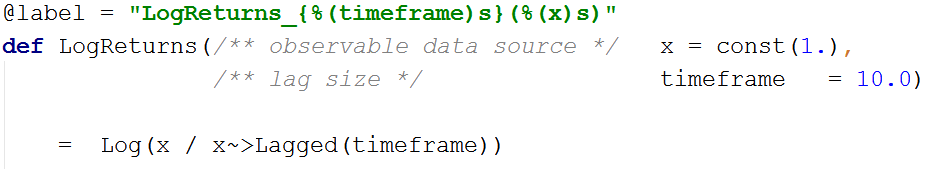
\includegraphics[width=1\linewidth]{logreturns.png}

Intrinsic functions represent simple modules and import classes from the target language into the DSL.
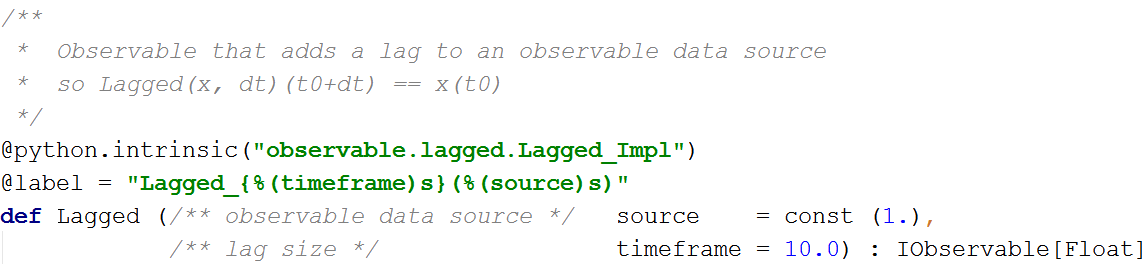
\includegraphics[width=1\linewidth]{lagged.png}

Types for parameters and return values are inferred automatically
\end{frame}
%------------------------------------------------
\subsection{Classes}
\begin{frame}
\frametitle{Classes}
Classes group functions and share fields among them

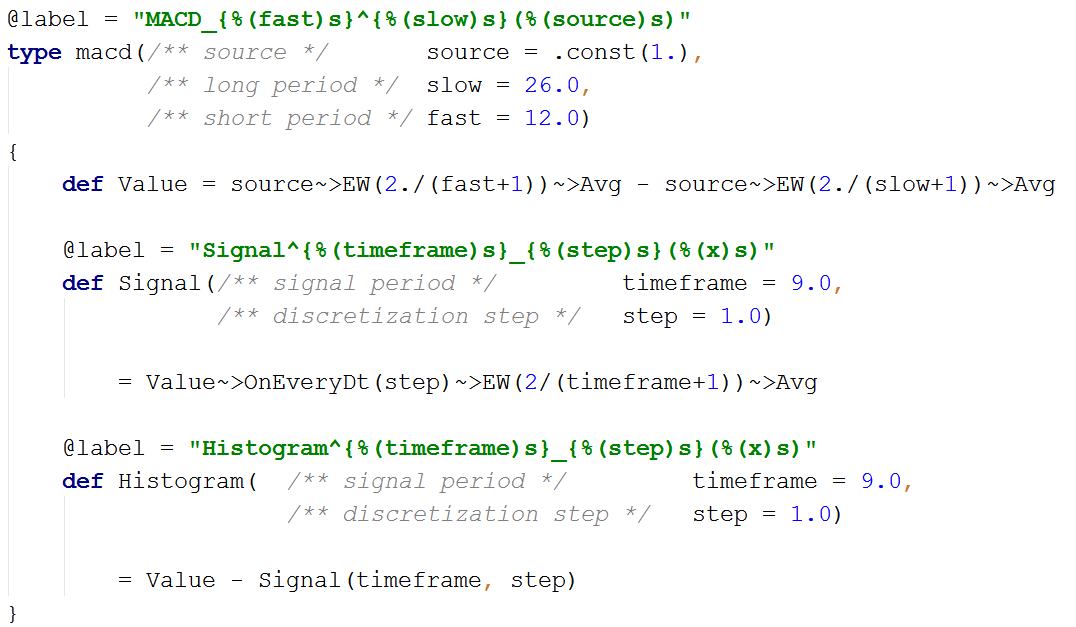
\includegraphics[width=1\linewidth]{macd.png}

\end{frame}
%------------------------------------------------
\subsection{Class Inheritance}
\begin{frame}
\frametitle{Class Inheritance}
To stimulate code re-use classes may derive from other classes

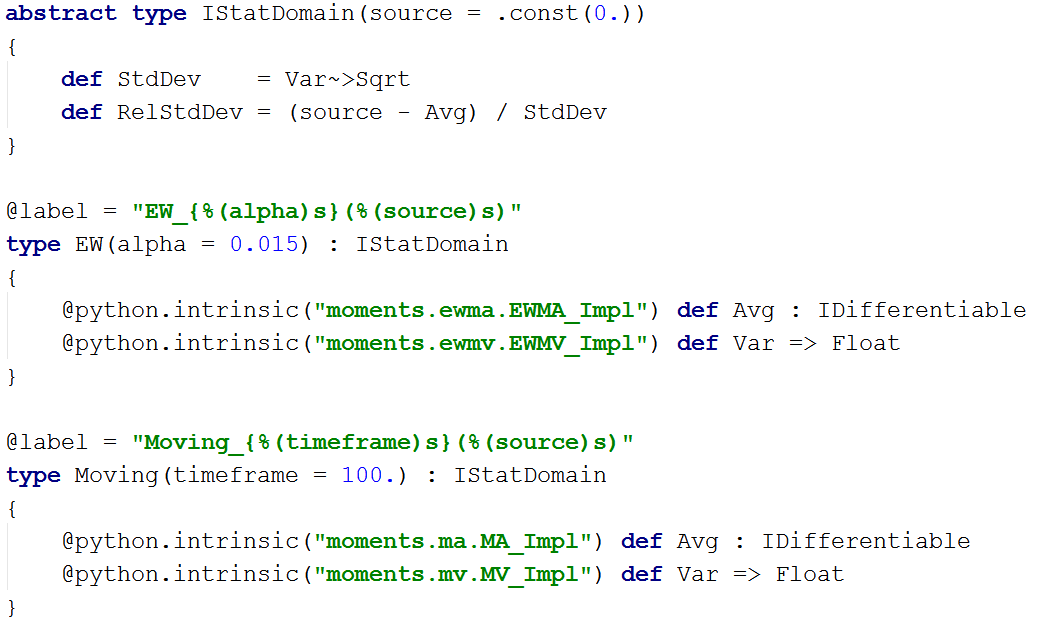
\includegraphics[width=1\linewidth]{moments.png}
\end{frame}
%------------------------------------------------
\subsection{Example}
\begin{frame}
\frametitle{Example: Signal Side Strategies}
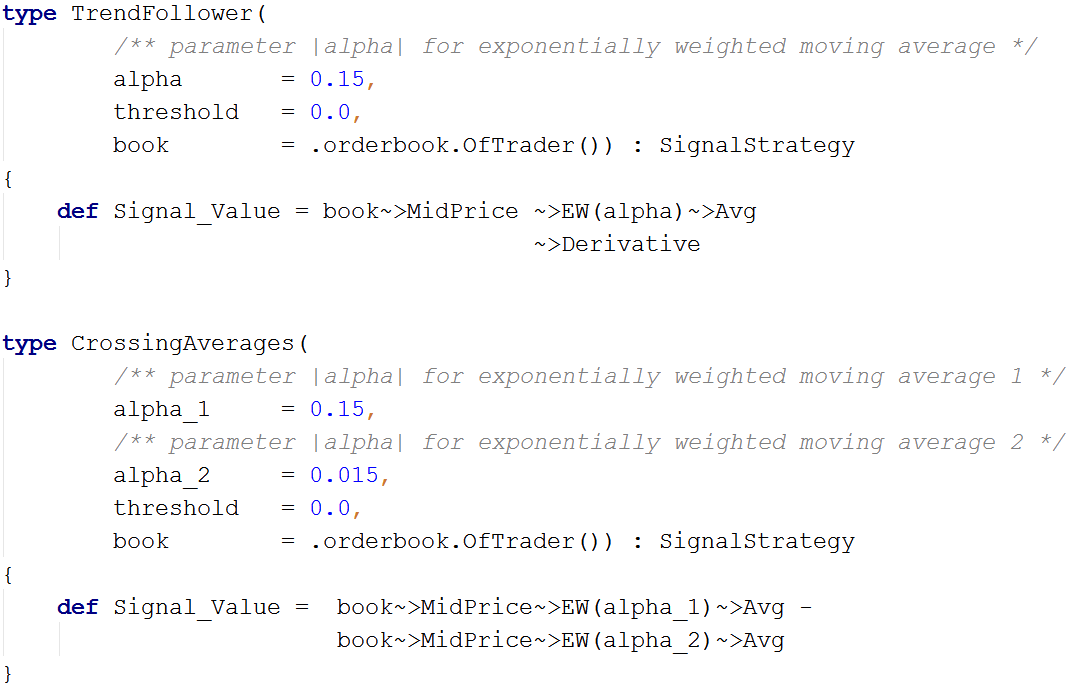
\includegraphics[width=1\linewidth]{side_strategies.png}
\end{frame}
%------------------------------------------------
\begin{frame}
\frametitle{Example: Signal Side Strategies Base}
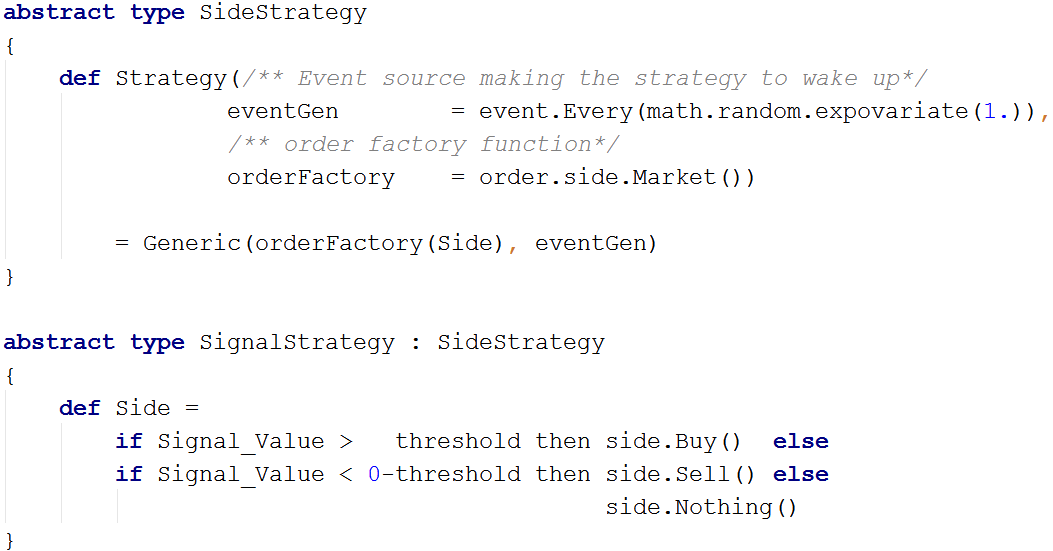
\includegraphics[width=1\linewidth]{side_strategies_base.png}
\end{frame}
%------------------------------------------------
\subsection{Summary}
\begin{frame}
\begin{itemize}
\item Developed at the Chair of Quantitative Finance at \'{E}cole Centrale Paris
\item Source code and documentation can be found at   \textcolor[rgb]{0.00,0.50,0.75}{\href{https://github.com/fiquant/marketsimulator}{https://github.com/fiquant/marketsimulator}}
\item OS supported: Linux, Mac OS X, Windows
\item Browsers supported: Chrome, Firefox, Safari, Opera
\item Requirements: Scala 10.2, Python 2.7 (Flask, NumPy, Pandas, Blist, Veusz).
\item Translator from the DSL into optimized C++ code is to be developed.
\item Many parts of the compiler can be re-used to create languages in other domains.
\end{itemize}

\end{frame}

\begin{frame}
\Huge{\centerline{Thank you for your attention!}}
\end{frame}

%----------------------------------------------------------------------------------------

\end{document} 